\chapter{Implementation and discussion} \label{chap: Result}

In order to verify the feasibility of the methodologies from chapter \ref{chap: Meth}, 
performance testing based on assumptions and two industrial uses cases 
are done and their results will be performed and discussed in this chapter. 
Again, the tests will also be divided into internal (\ref{chap: Result-Internal}) 
and external (\ref{chap: Result-External}) part, referring to those in chapter \ref{chap: Meth}.

\section{Internal}\label{chap: Result-Internal}
For the internal \gls{mas}, multiple tests are performed on the agent 
communication system. That means, the messages 
will be passed through the \gls{ca} under WebSocket architecture. 
Various tests will be done and the test results will be discussed later in section 
\ref{chap: Result-WS}. 
In addition to the performance testing of WebSocket architecture alone, 
a comparison between WebSocket and RestFUL API will be done to verify the feasibility 
of WebSocket. 
Finally, tests relevant to packets prioritization will be performed to close 
the sections. 


\subsection{Test results of WebSocket in various performance testing including worst case scenarios} \label{chap: Result-WS}

After the construction a \gls{mas} under WebSocket, the speed, robustness, 
reliability and application size of the system will be examined by 
performance tests. 

\subsubsection{Increasing client numbers}
In real world, the number of clients will greatly influence the performance of 
server. Assume that all agents serve as clients and \gls{ca} as a central server. 
  

By handling an increasing number of connection requests, and the growing demands 
of data processing capacity, the average total delay with or without process time can be 
roughly described as an overall increasing pattern. However, it does not necessarily 
need to be linear based on several reasons. In exercise, concurrent programming 
will speed up the processing for a large computation problem. As depicted in 
fig.\ref{fig: proportional-clients}, the average process time from one to ten 
clients is decreasing with a better utilization of the CPU power due to 
concurrent processing. However, by further increasing the clients number, the 
speedup will be limited by CPU cores number. Assume that a CPU has 8 core, 
and each core can handle 2 threads, it will have in total 16 threads to perform tasks.
In WebSocket based \gls{mas} program, the asynchronous I/O framework asyncio is used 
to handle the coroutines execution in order to better utilize the threads power.
Therefore, the asyncio is potentially more suitable for larger computational tasks 
compared to synchronous single thread programming.

Obviously there is a limit of the clients number to prevent system breakdown. 
With one server handling all clients at once, there is a system timeout problem of 
the server when the clients number reaches 1000. Therefore, 
distributing clients with more servers becomes a possible solution. 


\begin{figure}[htb]
    \begin{subfigure}[b]{0.49\textwidth}
        \centering
        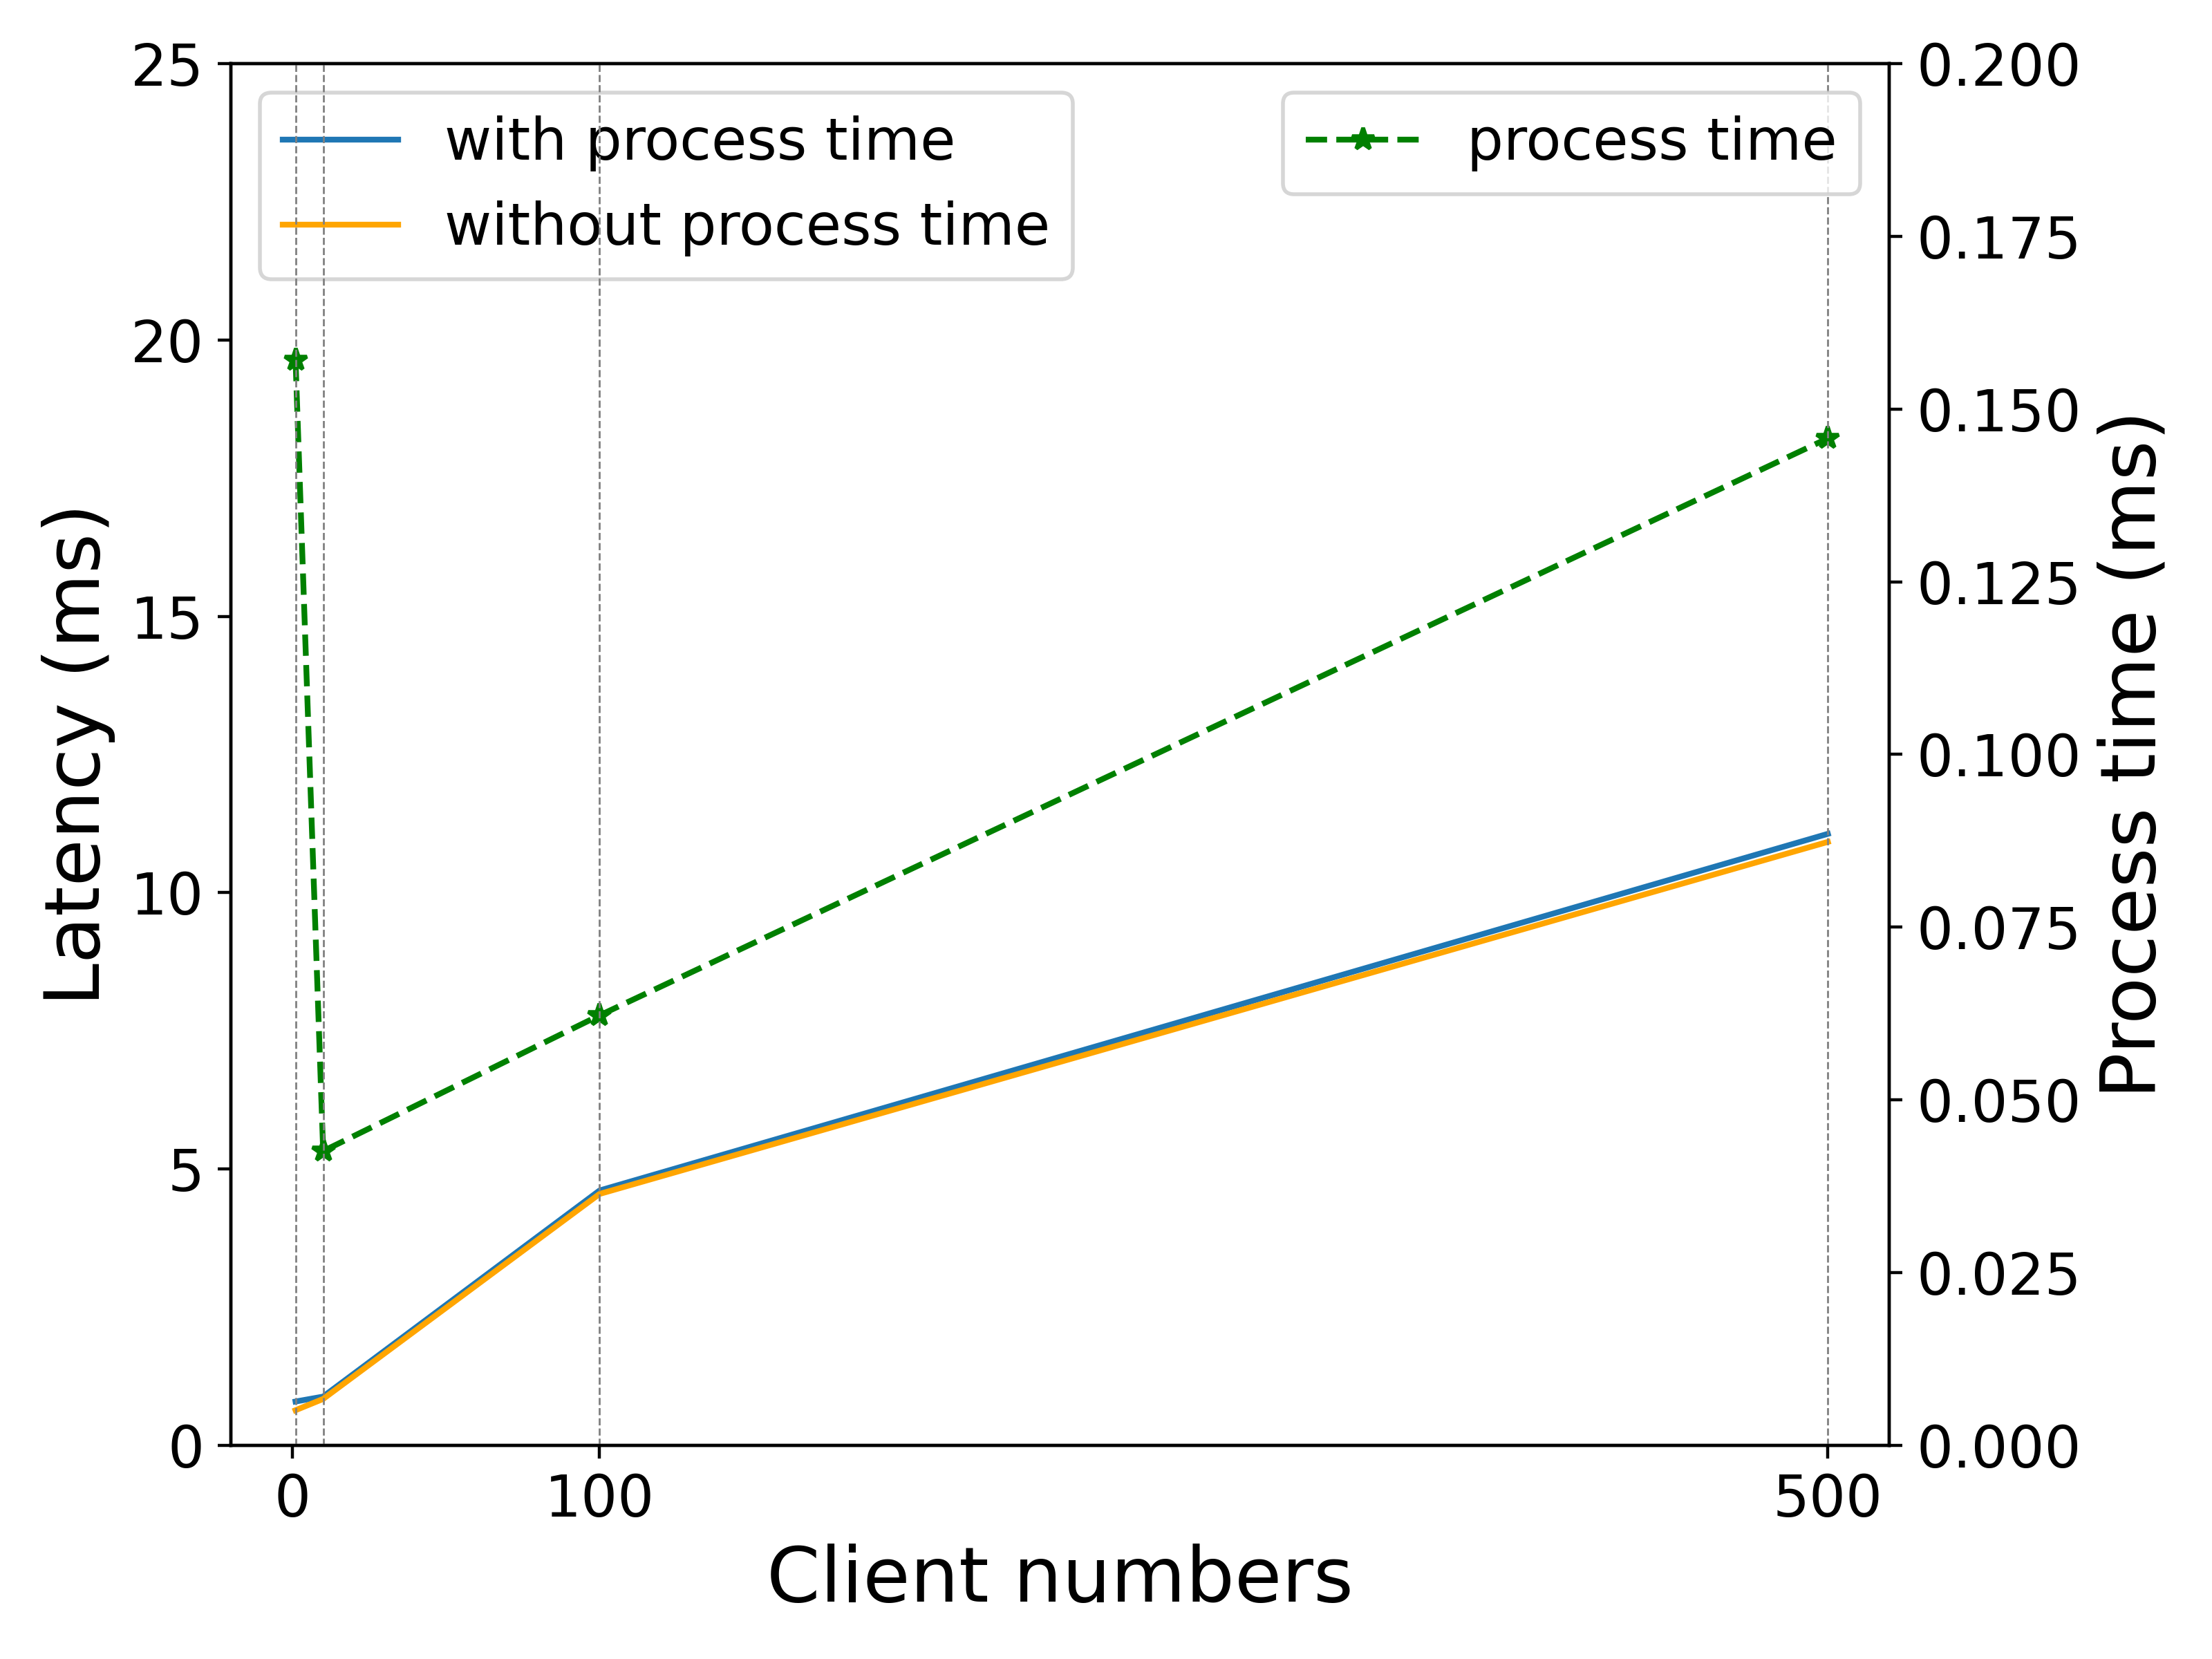
\includegraphics[width=\textwidth]{figures/tests/Average_string_messages_sending_time_of_100_tests_of_diff_client_numbers.png}\hfill 
        \caption{} \label{fig: proportional-clients-a}
    \end{subfigure}
    \begin{subfigure}[b]{0.49\textwidth}
        \centering
        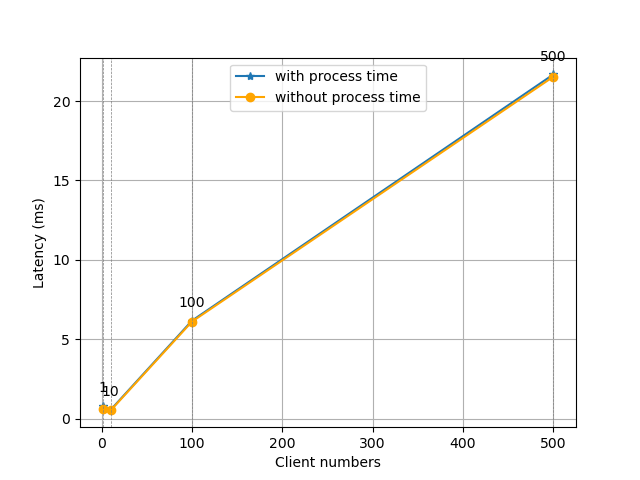
\includegraphics[width=\textwidth]{figures/tests/Average_string_messages_receiving_time_of_100_tests_of_diff_client_numbers.png}\hfill 
        \caption{} \label{fig: proportional-clients-b}
        \end{subfigure}
    \caption{Average delay of sending a string message 100 times 
    to a clientR from 1, 10, 100 or 500 clients separately. (a) Messages sent forward, 
    and (b) response messages from clientR. 
    \label{fig: proportional-clients}}
\end{figure}


\subsubsection{Increasing server numbers}
Under the same condition where 1000 clients are sending and receiving messages from 
a clientR, the messages will be separated this time to two or three groups, with 
each passing through different servers. Limited by the hardware configuration 
for the external routing solutions according to fig.\ref{fig: NSConceptual}, only 
maximal three servers can be used for the test. However, several assumptions 
can be made based on the results from fig.\ref{fig: proportional-servers}. 


\begin{figure}[htb]
    \begin{subfigure}[b]{0.49\textwidth}
        \centering
        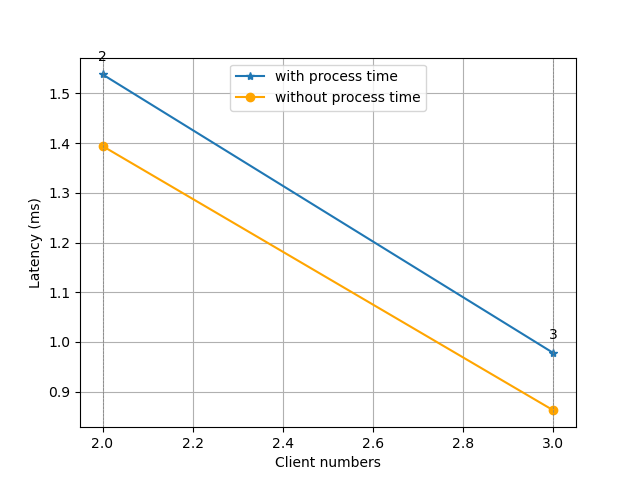
\includegraphics[width=\textwidth]{figures/tests/Average_string_messages_sending_time_of_100_tests_diff_server_numbers.png}\hfill 
        \caption{} \label{fig: proportional-servers-a}
    \end{subfigure}
    \begin{subfigure}[b]{0.49\textwidth}
        \centering
        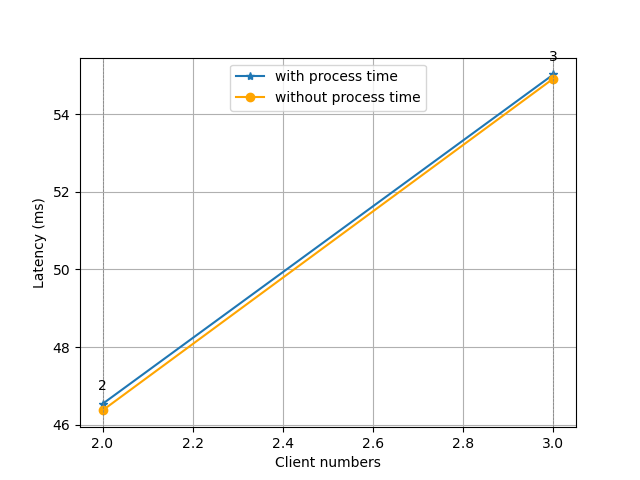
\includegraphics[width=\textwidth]{figures/tests/Average_string_messages_receiving_time_of_100_tests_diff_server_numbers.png}\hfill 
        \caption{} \label{fig: proportional-servers-b}
        \end{subfigure}
    \caption{Average delay of sending a string message 100 times 
    to a clientR from 1000 clients through 2 or 3 servers separately. (a) Messages sent forward, 
    and (b) response messages from clientR. 
    \label{fig: proportional-servers}}
\end{figure}

The latency reduction with an additional server according to 
fig.\ref{fig: proportional-servers-a} proves that, by introducing more servers 
to the system, the limited productive resources should be better utilized 
for frequent clients interactions. However, not as expected, the latency of 
clientR sending response messages back is much larger in \ref{fig: proportional-servers-b}.
The reason may be also relevant to the CPU consumption. Because of the high 
occupation of the CPU power when more than one servers are running in the same 
device, the loads between each process might be unbalanced. 
But overall this should be further verified with more servers involved in the 
future.

\subsection{Test results of WebSocket and RESTful API} \label{chap: Result-RestFUL_WS}

\subsection{priority tests of WS server in diff. performance testing} \label{chap: Result-priority}

\section{External}\label{chap: Result-External}

\subsection{Test results of DTagents related to Azure Digital Twin} \label{chap: Result-DT}